%!TEX root = ../thesis.tex
%*******************************************************************************
%*********************************** First Chapter *****************************
%*******************************************************************************

\chapter{Introduction}  %Title of the First Chapter


\section[Background]{Background}

Neuromorphic computing aims to bridge the gap between neuroscience and artificial intelligence by emulating the structural and functional principles of biological neural systems. At the heart of this vision is a pressing research question: how can we implement biorealistic learning on memristive networks to develop energy-efficient, scalable and adaptive computing architectures? Addressing this question requires a multidisciplinary approach, combining insights from neurobiology, electronic materials science and computational modelling. \\

\noindent Traditional von Neumann architectures \cite{von1993first}, characterised by their separation of memory and processing units, struggle to efficiently handle tasks that the human brain performs effortlessly, such as pattern recognition, sensory integration, and decision making. In contrast, the brain achieves these feats with remarkable energy efficiency and adaptability, in part due to the tightly coupled nature of computation and memory in its neural circuits. Mimicking these biological characteristics in silicon and emerging nanotechnologies has become the guiding principle of neuromorphic engineering \cite{saighi2015plasticity}. \\

\noindent Recent advances in memristive technologies have reignited interest in neuromorphic computing. Memristors, or memory resistors, are two-terminal non-volatile devices that can emulate synaptic plasticity by adjusting their conductance based on the history of voltage and current applied. This property lend itself to naturally support learning rules such as Hebbian learning \cite{hebb2005organization} and spike-timing-dependent plasticity (STDP) \cite{markram1997regulation}. When arranged in crossbar arrays, memristors offer a promising platform for in-memory computation, which can significantly reduce the power and latency associated with traditional data transfer bottlenecks. \\

\noindent This chapter presents a comprehensive discussion of biorealistic learning mechanisms and their physical realisation on memristive networks. By grounding the discussion in the neuroscientific principles that underlie learning and cognition, the chapter aims to elucidate how these biological processes can be abstracted and implemented in hardware. \\

\noindent The chapter begins with an overview of the biological basis of computation, providing an essential neuroscience primer. It then moves to device-level considerations, discussing the properties of memristive devices and their integration into neuromorphic architectures. Throughout, the emphasis is on aligning computational models with biological fidelity, while navigating the constraints and opportunities offered by emerging nanotechnologies.

\section[Neuroscience Primers]{Neuroscience Primers}

\noindent Computational neuroscience employs a computational methodology to elucidate the mechanisms underlying brain function. This entails not only identifying the computations performed by the brain but also understanding the interactions between brain elements, such as neurons and synapses, that facilitate these computations.\\

% \noindent The field of computational neuroscience has traditionally adopted a bottom-up approach, commencing with the study of individual neurons and subsequently examining how these can be integrated into progressively larger networks, ultimately leading to the emergence of meaningful behaviour. \\

% \noindent In contrast, psychology and cognitive science have adopted a more top-down approach, commencing with the observation of animal behaviour and subsequently attempting to elucidate the brain mechanisms underlying these behaviours in terms of the higher-level functions of large brain areas. \\

% \noindent This distinction has resulted in a historical focus on developing comprehensive mathematical models of individual neurons and small- to medium-sized networks in computational neuroscience. Recently, however, there has been a convergence with other fields, leading to the creation of neurally detailed models capable of reproducing organism-level behaviors. \\

\noindent The brain is capable of performing a vast array of computations, with the fundamental units of the brain generally considered to be neurons and synapses. In the context of the nervous system, a synapse is defined as a structure that is capable of facilitating the transfer of an electrical or chemical signal from a presynaptic neuron to a postsynaptic neuron. \\

% \noindent In the case of a chemical synapse, the occurrence of a spike in the presynaptic neuron will result in the stimulation of the release of a chemical substance known as a neurotransmitter. Subsequently, the neurotransmitter will migrate to bind with the receptors in the membrane of the postsynaptic neuron. \\

% \noindent The effects of different neurotransmitters vary, exerting excitatory or inhibitory effects on the postsynaptic neurons. Many receptors contain different ion channels, which permit ions to flow between the inside and outside of the membrane, thereby generating an excitatory postsynaptic current (EPSC) or an inhibitory postsynaptic current (IPSC). \\

\noindent This section provides a concise overview of the relevant biological details, in addition to the concepts and models from computational neuroscience that are employed or expanded upon in this study. These details provide invaluable preliminary information for accurately modelling the implementation of silicon oxide device-based neuromorphic hardware and bio-inspired computing. \\

\noindent 
In addition to the fundamental biological details that are pertinent to the subject under discussion, the section provides information both at the neural level and at the network level. It is important to acknowledge that the models outlined in this study are comparatively rudimentary when placed in contrast to the substantial corpus of evidence that has been amassed on the neural system. This extensive body of evidence \cite{kandel2000principles}, constitutes the preponderance of neural data concerning these domains. Consequently, this section presents only the most fundamental biological facts relevant to the present work.


\subsection[Neuron Anatomy and Electrophysiology]{Neuron Anatomy and Electrophysiology}

\noindent  A neuron is a specialised biological cell that processes and transmits information through electrical and chemical signals \cite{mel1994information}. They represent only one of the numerous cell types within the brain, yet they are the most frequently discussed due to their status as the primary computational entities. Their fundamental function is relatively straightforward: neurons receive input from other neurons, and if that input is sufficiently stimulating, they will fire an action potential (also known as a spike), which propagates to other neurons.\\

\noindent Figure \ref{fig:1a} illustrates the basic structure of a neuron. Neurons can be subdivided into three principal parts: the dendrites, the cell body (soma), and the axon. Neurons receive input currents via their dendrites, which then transmit or channel this into the cell body, called the soma. When a neuron spikes, it sends current down its axon, which results in the release of neurotransmitter(s) at the synapses. These are connections from a neuron's axon to the dendrites of other neurons, and the neurotransmitter release causes dendritic input currents in these other connected neurons. \\

\begin{figure}[htbp!] 
    \centering    
    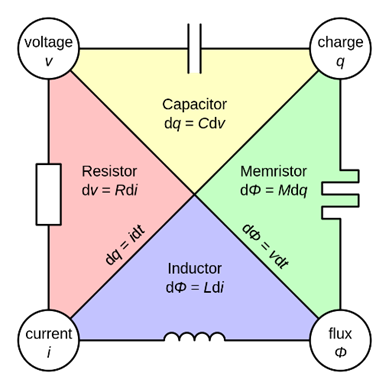
\includegraphics[width=0.5\textwidth]{Chapter1/Figs/1a.png}
    \caption[Labeled diagram of the neuron.]{Labeled diagram of the neuron, nerve cell that is the main part of the nervous system. A neuron's dendrites include synapses that allow it to accept input from other neurons. The dendrites carry current to the soma, which is where electrical charge is integrated. If the neuron membrane gets sufficiently polarised, an action potential (also known as a spike) travels down the axon. This causes neurotransmitters to be released at synapses, resulting in currents in the dendrites of postsynaptic neurons.}
    \label{fig:1a}
    \end{figure}

\noindent From a computational perspective, the soma represents the integration point for all incoming currents from dendrites \cite{polsky2004computational}, marking the initiation of the action potential generation process (Figure \ref{fig:1b}). When a neuron is at rest, the soma exhibits a negative charge. This is referred to as the resting voltage and is maintained by ion pumps that regulate the concentration of ions (predominantly sodium, $Na^+$, potassium, $K^+$, and calcium, $Ca^{+2}$) within the cell. \\


\noindent As the currents arrive from the dendrites, they initiate a process of depolarisation of the cell \cite{johnston1996active}. Once the voltage within the soma reaches a sufficient level, it initiates the opening of voltage-activated sodium channels, which permit the influx of sodium ions into the cell, further depolarising it. This process persists until the electrical gradient resulting from the accumulation of sodium ions reaches a point where it is no longer in equilibrium with the chemical gradient caused by the imbalance of sodium within and outside the cell. This leads to a notable increase in the neuron's positive charge, exceeding the resting voltage. \\

\noindent Furthermore, this substantial depolarisation also activates voltage-gated potassium channels, which subsequently permit the release of potassium ions from the cell, thereby facilitating repolarisation. Concurrently, the sodium channels undergo inactivation. The opening of potassium channels ultimately results in the cell reaching a voltage below its resting level, a state known as hyperpolarisation. The sodium channels remain inactivated and the potassium channels remain open for a period of time following the spike. \\

\begin{figure}[htbp!] 
    \centering    
    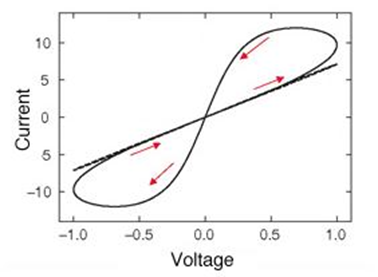
\includegraphics[width=0.45\textwidth]{Chapter1/Figs/1b.png}
    \caption[Spiking dynamics of a neuron.]{The action potential and the underlying conductance and currents with respect to time \cite{squire2012fundamental}. It should be noted that the increased conductance for $Na^+$ (and its inward flow) is associated with the rising phase of the action potential, whereas the slower increase in conductance for $K^+$ (and its outward flow) is associated with repolarisation of the membrane and with afterhyperpolarisation. The reduction in $I_{Na}$ before the peak of the action potential (even though $G_{Na}$ is still high) is due to inactivation of the Na+ channels.}
    \label{fig:1b}
\end{figure}

\noindent The combination of these factors renders it almost impossible for the neuron to fire during this time; this is referred to as the absolute refractory period. The change in ionic concentrations within the cell is relatively minor during a single spike, but over the course of numerous spikes, the ion pumps are required to maintain the optimal concentrations of sodium and potassium. Other currents, most notably calcium currents, are present in some neurons. \\

\noindent The rapid depolarisation associated with an action potential not only causes an increase in the somatic voltage potential, but also results in partial depolarisation of the axon segments situated in closer proximity to the soma. This results in the opening of sodium channels in that part of the axon, which in turn causes further depolarisation and the opening of sodium channels in the subsequent section of the axon. In this way, the somatic spike triggers a voltage wave that travels down the axon, eventually leading to the release of neurotransmitter(s) from synaptic vesicles situated near the ends of the axon. \\

% \noindent Axons are responsible for transmitting long-range signals in the brain, and thus exhibit considerable variation in length, contingent on whether a given neuron is connected to neighbouring neurons or to neurons situated in a different brain region. To facilitate long-range transmission, axons are coated in myelin, a substance composed mainly of lipids and thus a good electrical insulator.\\

% \noindent This enables the propagation of current down the axon. The high proportion of fat makes myelin white; bundles of axons are responsible for the "white matter" parts of the brain. In contrast, the "grey matter" is composed mainly of neuron dendrites, somas, and short-range axons.\\

% \noindent Dendrites are thin processes that extend away from the soma to connect to the axons of other neurons \cite{johnston1996active}. They serve to transmit current from synapses with other neurons to the soma. Initially, it was thought that they only conducted current passively; however, research has demonstrated that they possess active conductance mechanisms that are analogous to those involved in spike generation and propagation down an axon.\\

% \noindent Dendrites are also traditionally considered to act in a linear manner, whereby inputs from numerous synapses are accumulated over time and space. This remains a prevalent assumption in numerous computational models. However, recent studies have demonstrated that the summation of signals in dendrites is more intricate, exhibiting a combination of linear and nonlinear (sigmoidal) elements.\\

% \noindent Neurons are connected to one another by synapses, which facilitate the connection between the axon of the presynaptic neuron and a dendrite of the postsynaptic neuron. Upon the occurrence of a spike in the presynaptic neuron, an electrical pulse is transmitted along the axon, reaching the presynaptic terminals of all synapses situated along its length. The synaptic vesicles, which are filled with neurotransmitter, are located at the terminals. \\

% \noindent When an electrical pulse is generated, it causes the vesicles to release neurotransmitter into the synaptic cleft, which is the narrow space between the presynaptic terminal and the postsynaptic terminal. This neurotransmitter then activates receptors on the postsynaptic terminal, which open and permit the flow of current into the postsynaptic cell. The specific neurotransmitter utilized by the synapse is contingent upon the presynaptic neuron. \\

\noindent It has been established that all synapses located along a neuron's axon are responsible for the release of a singular neurotransmitter or a combination of neurotransmitters. This phenomenon is commonly referred to as Dale's principle. At the time of its development, Dale's principle was based on the assumption that each neuron produced a single type of neurotransmitter. Nevertheless, evidence of cotransmission was only discovered subsequently \cite{burnstock2004cotransmission}. It was understood that neurotransmitters can only be either excitatory or inhibitory,in relation to different postsynaptic cells.

\subsection[Spiking Neuron Dynamics]{Spiking Neuron Dynamics}

\noindent In recent times, the number of available neuron models has proliferated. The models currently in use in the literature range from the simplest possible rate-neuron model, namely binary threshold units \cite{stocks2001information}, to complex multi-compartmental models that account for detailed dendritic morphologies \cite{markram2015reconstruction}. In the context of large-scale neural models aiming to reproduce high-level behaviours, single-compartment neuron models remain the prevailing approach. \\

\noindent These models treat the neuron as a single electrical compartment, combining the dendrites, soma, and axon. In contrast, multi-compartmental models represent the neuron as comprising multiple electrical compartments, with equations that describe the influence of activity in one compartment on that of another. By modelling the spike separately from the rest of the neural dynamics, it is possible to separate time scales, thereby avoiding the need for additional computational resources to model the spike trajectory \cite{abbott1999lapicque}. \\

% \noindent The number of compartments in a model can vary considerably, from a minimalistic two-compartment structure, typically comprising one for the dendrites and one for the soma, to a more elaborate configuration comprising thousands of compartments. \\

% \noindent The number of compartments in a model is directly proportional to the amount of computing power required for simulation and the complexity of the resulting behaviour. For these reasons, models that seek to reproduce behaviour predominantly utilise either single-compartment neurons or simpler models that do not model the electrical activity of the neuron at all. \\

% \noindent Single-compartmental neuron models can be classified according to two key dichotomies: firstly, the rate-based versus spike-based dichotomy; and secondly, the static versus dynamic dichotomy. The distinction between rate-based and spiking neuron models concerns the nature of the output: is it a continuous value, represented by a firing rate, or a discrete value, represented by a spike.\\

% \noindent The distinction between static and dynamic models concerns the extent to which the model exhibits internal dynamics. In a static model, the output at a given point in time is independent of the neuron's past history and solely contingent on its instantaneous input. In contrast, a dynamic model allows for some degree of dependence on the neuron's past trajectory.\\

% \noindent Dynamic neuron models possess a state, which is to say, internal variables that evolve over time and are not directly computable from the present input to the model. They are typically expressed using differential equations. In contrast, static models output a function of the current input only; thus, they do not require differential equations to express them. \\

% \noindent It is important to note that the distinction between static and dynamic neurons does not necessarily refer to whether the neuron is being used as a static nonlinearity, evaluated at a single point in time on an input value, or as a dynamic nonlinearity, evaluated over a period of time on an input signal. \\

% \noindent Static neurons can be evaluated dynamically by evaluating them independently at each successive point in time on the input value. In contrast, there is no general method for evaluating dynamic neurons statically, as their input at any given point in time is contingent upon their internal state, which is a dynamic process that evolves over time. \\

% \noindent In some cases, it is possible to determine a firing rate response curve, also known as an I-F response curve or rate response function, for dynamic neuron models. This curve maps every constant value of the input current to a constant firing rate output. This can be determined analytically or empirically by applying a constant input current and measuring the rate of the output spikes, this can even be done in real neurons in vitro. \\

% \noindent However, many neuron models will not output spikes at a constant rate, even for a constant input, due to changing internal dynamics. In such cases, the rate-response function only captures part of the model, and will be different depending on the state of the model and how it is measured or calculated. \\

% \begin{table}[]
% \caption{Neuron Model Dichotomies.}
% \centering
% \begin{tabular}{|c|c|c|}
% \hline
%                  & \textbf{Rate}                                                                  & \textbf{Spiking}                                             \\ \hline
% \textbf{Static}  & Sigmoid Rate LIF                                                               & Poisson Spiking                                              \\ \hline
% \textbf{Dynamic} & \begin{tabular}[c]{@{}c@{}}Adaptive Rate LIF\\ Sigmoid with State\end{tabular} & \begin{tabular}[c]{@{}c@{}}Hodgkin-Huxley\\ LIF\end{tabular} \\ \hline
% \end{tabular}
% \label{table:4a}
% \end{table}

% \noindent Table \ref{table:4a} illustrates the manner in which a small selection of neuron models align with these dichotomies. In the static rate category, the models in question take in a continuous value and output a continuous function of that value. This encompasses the majority of non-linearities employed in machine learning (such as sigmoids or rectified linear units), in addition to the analytic firing rate for the LIF neuron model. \\

% \noindent In the static spiking category, models are characterised by the output of a discrete (binary) function of their continuous input. This category is primarily composed of Poisson-spiking neurons, which fire probabilistically based on their instantaneous firing rate. This implies that the probability of firing at a given time is independent of past firings. Furthermore, Poisson spiking can be applied to a dynamic rate model, whereby the probability of spiking is independent, but the spike rate is a dynamic process. \\

% \noindent Dynamic rate models possess an internal state that influences their continuous output, in addition to the input. This encompasses the analytic LIF rate model with adaptation, which possesses an intrinsic adaptation parameter that increases when the neuron is active and discounts the firing rate. Furthermore, the category encompasses sigmoid neuron models that possess an underlying voltage that is dynamically correlated with the neuron inputs \cite{lillicrap2016random}. \\ 

% \noindent The dynamic spiking category also includes the LIF neuron model, the Hodgkin-Huxley model, and more intricate multi-compartmental models. Within the category of spiking models, a distinction can be made between those that output instantaneous spikes (e.g., LIF) and those that output spikes that vary across time (e.g., Hodgkin-Huxley). Recently, another study have employed such models in the context of deep networks \cite{guerguiev2017towards}, subject to biological constraints. \\

% \noindent Another potential distinction can be made between models that output stereotyped spikes, where the size of each spike is identical, and those that output variable-sized spikes. Models of cortical neurons that output instantaneous spikes (e.g., LIF) almost invariably output stereotyped spikes. This is due to the fact that spikes in cortical neurons are almost identical in terms of magnitude, duration, and shape.\\

% \noindent It is widely believed that none of these factors carry information. Even among models that have spikes that vary across time (e.g., Hodgkin-Huxley), the spike magnitude, duration, and shape are quite consistent between spikes. Therefore, the majority of spiking cortical neuron models exhibit stereotyped spikes. \\

% \noindent By modelling the spike separately from the rest of the neural dynamics, it is possible to separate time scales, thereby avoiding the need for additional computational resources to model the spike trajectory, which is characterised by stereotyped details of little interest \cite{abbott1999lapicque}. \\

\begin{figure}[htbp!] 
    \centering    
    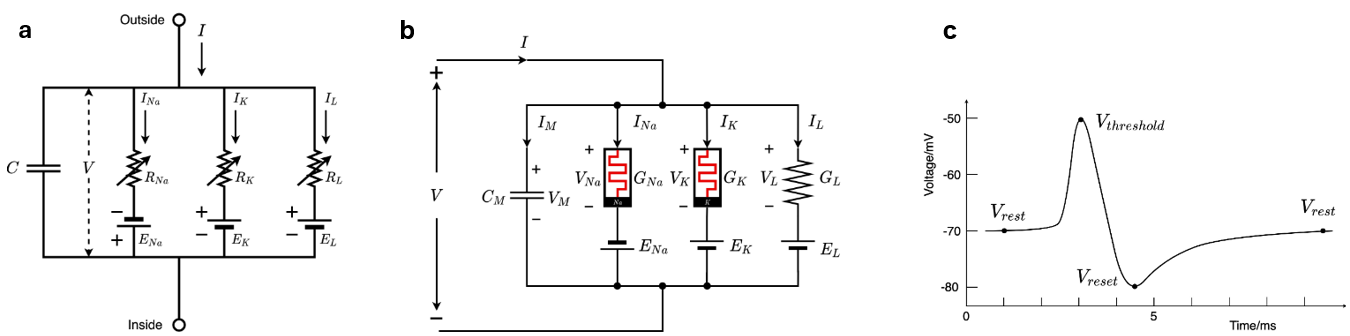
\includegraphics[width=1\textwidth]{Chapter1/Figs/1c.png}
    \caption[Hodgkin-Huxley neuron model.]{Hodgkin-Huxley neuron model. (a) An equivalent circuit for the HH models \cite{hodgkin1952quantitative}. (b) An equivalent circuit for memristive HH model \cite{chua2012hodgkin}. (c) An action potential waveform, which demonstrates the resting, threshold, and reset potentials. }
    \label{fig:1c}
\end{figure}

\noindent A significant proportion of the most influential findings in computational neuroscience are based on mathematically detailed models of neuronal functioning. One of the most renowned of these is the Hodgkin-Huxley model of the squid giant axon \cite{hodgkin1952quantitative}. the Hodgkin–Huxley (HH) model is one of the most widely used, comprising a set of nonlinear differential equations that accurately approximate the electrical signals of neurons \cite{chua2012hodgkin}. \\

\noindent Figure \ref{fig:1c}(a) depicts the HH neural model, wherein the time-varying nonlinear conductor $R_{Na}(GNa)$ and $R_K(G_K)$ represent the sodium and potassium channels, respectively, while the linear conductor $R_L(G_L)$ simulates leak channels and $C$ models the membrane of a neuron. The equations of the HH model are presented below: 
\begin{align}
    C \frac{dV_m(t)}{dt} = I_C(t) + \sum_{k}^{}I_k(t) \label{eq:1.1} 
\end{align}

\noindent In this context, $V_m$ represents the membrane potential. $\sum_{k}^{}I_k(t)$ denotes the sum of the ionic currents flowing into the neuron. This can be formulated by three ion currents, as follows:
\begin{align}
    \sum_{k}^{}I_k &= C_m \frac{dV_m}{dt} + G_Kn^4(V_m - V_K) + G_{Na}m^3(V_m - V_{Na}) + G_L (V_m - V_L) \label{eq:1.2} \\
    \frac{dn}{dt} &= \alpha_n(V_m)(1-n)-\beta_n(V_m)n \label{eq:1.3} \\
    \frac{dm}{dt} &= \alpha_m(V_m)(1-m) - \beta_m(V_m)m \label{eq:1.4} \\
    \frac{dh}{dt} &= \alpha_h(V_m)(1-h)-\beta_h(V_m)h \label{eq:1.5}
\end{align}

\noindent The reversal potentials $V_K$, $V_{Na}$, and $V_L$ are the three parameters in question. The rate constants $\alpha_i$ and $\beta_i$, which depend on the membrane potential, describe the behaviour of the $i^{th}$ ion channel. The maximal value of the conductance is represented by $G_K$, $G_{Na}$, and $G_L$. \\

\noindent Finally, the dimensionless quantities \textit{n}, \textit{m}, and \textit{h}, which lie between 0 and 1, are associated with three ion channels. In order to achieve the optimal fit for human action potentials, the HH model is reduced by setting the leakage channel conductance to $G_L = 0$  \cite{noble1962modification}.It has been demonstrated that $G_{Na}$ and $G_K$ are memristors \cite{chua1976memristive}, in the equivalent circuit in figure \ref{fig:1c}(b). \\

\noindent The integrate-and-fire (IF) neuron \cite{lapicque1907louis} constituted one of the earliest computational models of a neuron. This model was developed prior to the ability of researchers to measure the electrical and chemical changes occurring in a functioning neuron. It is based on the premise that the neuron membrane can be modelled as a capacitor that stores charge over time \cite{abbott1999lapicque}.\\

\noindent As the name suggests, the IF model exhibits two principal behaviours: The model integrates current over time, as would be expected of a capacitor, and fires when the voltage reaches a threshold. Furthermore, the model may or may not incorporate a leak term, which represents a resistor in parallel with the capacitor that permits the dissipation of charge over time. The model with a leak term is typically designated as the leaky integrate-and-fire (LIF) model. While the term "integrate-and-fire (IF) model" can be used interchangably. \\

\noindent To identify how the neuron's membrane voltage evolves over time and, based on this, to determine when the neuron spikes, the charge \textit{Q} across a capacitor is represented by $Q = V \times C$, where \textit{V} is the voltage across the capacitor and \textit{C} is the capacitance. By differentiating this with respect to time, the membrane voltage $\textit{V(t)}$ of the neuron is:
\begin{align}
    C \frac{dV(t)}{dt} = J(t) \label{eq:1.6} 
\end{align}

\noindent In this context, \textit{J(t)} represents the input current to the neuron over time, whereas \textit{C} denotes the membrane capacitance. The current here is the time derivative of charge. Equation \ref{eq:1.6} demonstrates that the IF neuron simply integrates the input current over time. It is still necessary to identify the point at which the neuron spikes. \\

\noindent This is achieved by defining a threshold voltage, $V_{th}$, which is exceeded when the voltage passes this threshold, resulting in the neuron firing. This is a fundamental principle in neurophysiology: once the neuron voltage passes a threshold, the neuron begins firing a spike, and once this firing process begins, it is almost impossible to reverse. \\

\noindent Once a neuron has fired a spike, the membrane voltage is reset to the resting potential, $V_{rest}$. This phenomenon can be attributed to physiological resetting procedures. Following the occurrence of a spike in a neuron, other ionic currents, typically potassium, are initiated, leading to a restoration of the membrane voltage towards the resting potential.\\

% \noindent Some integrate-and-fire models may also incorporate an absolute refractory period, defined as a time interval during which the voltage is maintained at the resting potential $V_{rest}$ following a spike. In cortical neurons, post-spike potassium currents are sufficiently strong to prevent another spike from occurring for a considerable duration. This time interval is referred to as the absolute refractory period. The model accounts for this by holding the membrane voltage at $V_{rest}$ for a duration equal to the absolute refractory period. \\

\noindent The leaky integrate-and-fire (LIF) model \cite{knight1972dynamics} incorporates an additional physiological factor: Neuron membranes are not perfect capacitors; rather, they slowly leak current over time, pulling the membrane voltage back to its resting potential. Therefore, the membrane is modelled as a capacitor and resistor in parallel, which allows for the neuron to exhibit a degree of "forgetting": in the absence of any input, the membrane voltage will return to its resting potential \cite{koch2004biophysics}. The LIF dynamics are captured by the following equation:

\begin{align}
C \frac{dV(t)}{dt} = J(t) - \frac{1}{R} (V - V_{rest}) \label{eq:1.7} 
\end{align}

\noindent In this model, \textit{R} represents the membrane resistance, and the remaining parameters are consistent with those of the IF model, with identical resetting procedure.\\

\noindent The LIF model comprises a number of parameters, including $C, R, V_{rest}$ and $V_{th}$. It is possible to normalise the model in order to reduce the number of parameters while maintaining the full dynamics of the original model. In particular, the model can be manipulated so that the normalised voltage lies within the range [0, 1], with a normalised resting potential of zero and a normalised firing threshold of one. Initially, Equation \ref{eq:1.7} is multiplied by R to give:

\begin{align}
    \tau_{rc} \frac{dV}{dt} &= RJ(t) - V + V_{rest} \label{eq:1.8} \\
    \tau_{rc} &= R \times C \label{eq:1.9} \\
    \bar{V} &= \frac{V - V_{rest}}{V_{th} - V_{rest}} \label{eq:1.10} \\
    \bar{V_{rest}} &= \frac{V_{rest}}{V_{th}} \label{eq:1.11} 
\end{align}

\noindent By substituting $\bar{V}$ and $\bar{V_{rest}}$ into equation \ref{eq:1.3} to give:


\begin{align}
    \tau_{RC}(V_{th} - V_{rest})\frac{d\bar{V}}{dt} &= RJ(t) - \bar{V}(V_{th} - V_{rest})
    \label{eq:1.12} \\
    \tau_{rc}\frac{d\bar{V}}{dt} &= \frac{R}{V_{th} - V_{rest}} J(t) - \bar{V} \label{eq:1.13} \\
    \tau_{rc} \frac{d\bar{V}}{dt} &= \bar{J}(t) - \bar{V} \label{eq:1.14} 
\end{align}

\noindent When the firing threshold for the new equation $\bar{V_{th}} = 1$, the voltage resets to $\bar{V_{rest}} = 0$, and $\bar{J}(t) = \frac{R}{V_{th} - V_{rest}} J(t)$. It can be observed that $\bar{J}(t)$ is merely a linear transformation of $J(t)$. Consequently, (\ref{eq:1.14}) retains the full dynamics of (\ref{eq:1.7}) for a scaled input, but with only one parameter, $\tau_{RC}$. \\

\noindent It should be noted that both $\bar{V}$ and $\bar{J}$ are unitless quantities. Conventionally, the unitless space is employed exclusively, and the quantities are often referred to simply as \textit{V} and \textit{J}, despite the fact that they are not voltages or currents. This simplifies the mathematical representation, without limiting the generality of the models. \\

\noindent (\ref{eq:1.14}) provides an exact description of the circumstances under which the model neuron will spike in response to a given input current, \textit{J(t)}. However, in some cases, it is sufficient to consider only the spike rate, that is, the number of spikes per second that the neuron will produce in response to a given input current. \\

\noindent In the case of the LIF model, it is possible to determine the analytical firing rate for a constant input current. This is achieved by calculating the inter-spike interval (ISI), which is the time between one spike and the next. The firing rate is then given by the inverse of the ISI. When a constant input current, $J(t) = j$, is provided, it is possible to solve (\ref{eq:1.14}) in order to find the neuron voltage over time. 
\begin{align}
    V(t) = (V(0) - j)e^{\frac{-t}{\tau_{rc}}} + j \label{eq:1.15}
\end{align}

\noindent In the absence of spikes, the objective is to ascertain the time required for the voltage to increase from$ V(0) = 0$ to $V(t) = 1$. This property will only occur if $j > 1$. Substitution into (\ref{eq:3.15}) and subsequent solution for \textit{t} yields:
\begin{align}
    t = - \tau_{RC} log \left( - \frac{1}{j} \right) \label{eq:1.16}
\end{align}

\noindent Incorporating the refractory period and performing the inversion, the spike rate \textit{r} for the LIF neuron is given by:
\begin{align}
    r &= \begin{cases}
    \frac{1}{t_{ref} - \tau_{RC} log \left( 1 - \frac{1}{j} \right)} & \text{ if } j > 1 \\ 
    0 & \text{ otherwise }  
    \end{cases} \label{eq:1.17}
\end{align}


\noindent The LIF model is one of the most widely utilised simplified neuron models \cite{lapique1907researches}. The simple equivalent model is illustrated in Figure \ref{fig:1d}(a). In this model \cite{stein1967frequency}, a resistor \textit{R}, connected in series with a \textit{DC} source $V_{rest}/V_{reset}$, is connected in parallel with a capacitor \textit{C}. A postsynaptic neuron receives a synaptic current \textit{I(t)}, generated by presynaptic spikes. \\

\noindent A proportion of the current \textit{I(t)} flowing into \textit{C} results in an increase in the membrane potential \textit{V(t)}. The charge leakage occurs via resistor \textit{R}. When \textit{V(t)} reaches a threshold value, the neuron generates a spike. Following the generation of a spike, the membrane potential is reset to the reset value. \\

\begin{figure}[htbp!] 
    \centering    
    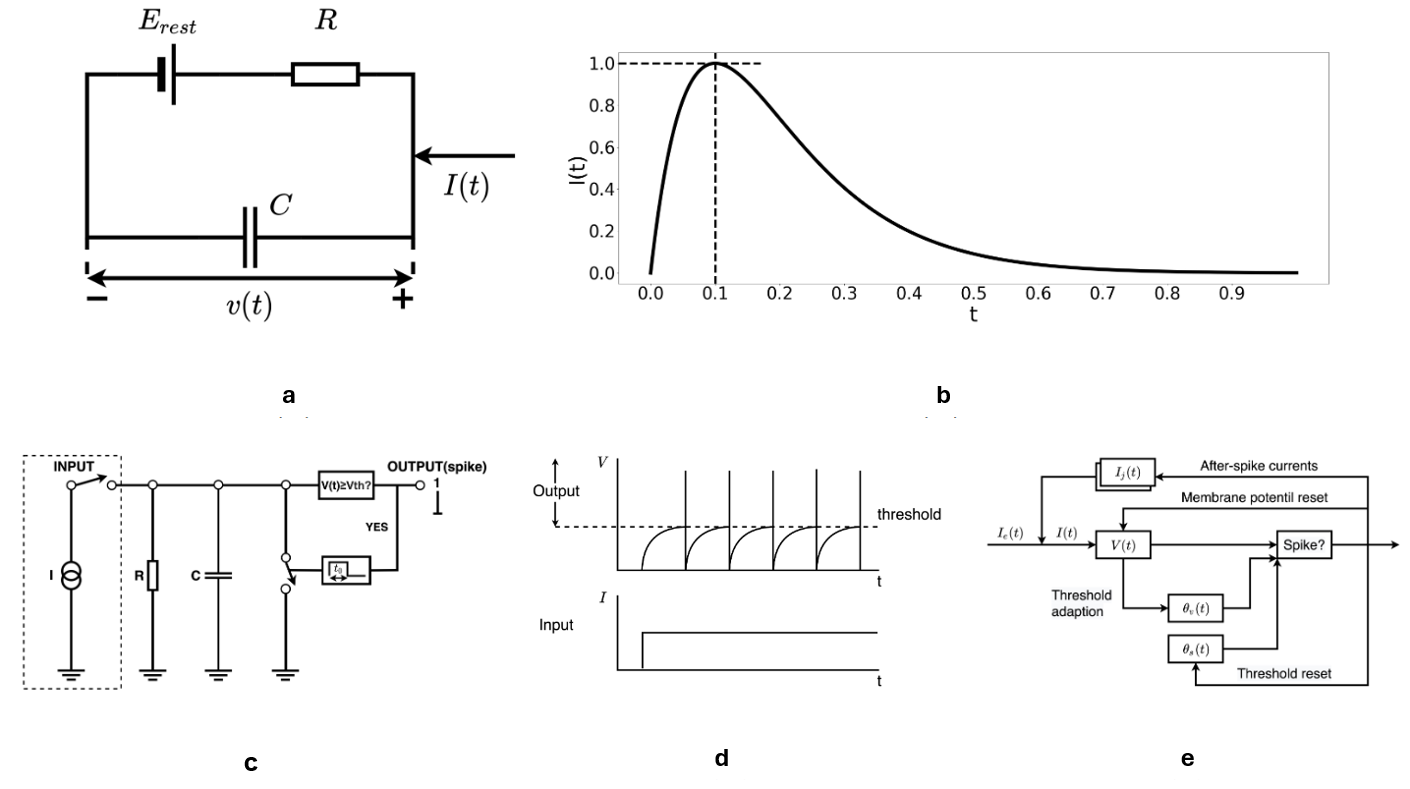
\includegraphics[width=0.8\textwidth]{Chapter1/Figs/1d.png}
    \caption[The Leaky Integrate-and-Fire neuron model.]{The LIF neuron model. (a) Schematic diagram of the LIF electrical model. (b) Input current in the form of an alpha function, $\tau_{\alpha} = 0.1, I_0 = 1$ (c) The LIF model allows for the control of spiking behaviour through a comparison of membrane potential and threshold at each time step. Upon the triggering of a spike, a voltage-controlled switch discharges C for a duration corresponding to the refractory period $t_0$ \cite{tal1997computing}. (d) A simulation of constant firing frequency for DC current input in which $t_0$ is hidden. DC input current and output spikes are both shown. (e) A generalised LIF model with threshold control \cite{teeter2018generalized}. }
    \label{fig:1d}
\end{figure}

\noindent In the absence of \textit{I(t)}, the voltage across \textit{C} is eventually settled at $V_{rest}$, representing the cell's resting potential. During the refractory period $t_0$, a neuron is incapable of spiking. Figure \ref{fig:1d}(c,d) illustrates the LIF neuron dynamics for the case of a \textit{DC} input current and a zero rest and reset potential, $E_{reset} = E_{rest} = 0$ \cite{tal1997computing}. \\

\noindent The input synaptic current, \textit{I(t)}, can be described by a time-varying alpha function. However, alternative functions may be employed, including "Instantaneous Rise and Single Exponential Decay," "Biexponential Functions," "Sawtooth," and "Pulse Function." The alpha synaptic current is modeled by Equation \ref{eq:3.15}, and the resulting plot is shown in Figure \ref{fig:4b}(b). \\

\noindent Nevertheless, Figure \ref{fig:3d}(a) lacks a circuit for resetting the system when the threshold is reached. In order to evaluate the inequality $V > V_{threshold}$, it is necessary to use an active circuit, such as a comparator. Upon reaching the threshold, the membrane potential must be reset in accordance with the illustration in Figure \ref{fig:3d}(d). Therefore, the LIF model's generalized version necessitates additional overhead, as illustrated in Figure \ref{fig:3d}(e). \\

% \noindent In the generalized LIF model, the reset behavior necessitates external control to pull down the membrane potential below the resting potential. This external control requires intricate, active circuits comprising MOS transistors, resistors, and even a silicon-controlled rectifier (SCR), which represents a significant drawback in a neuromorphic system due to its substantial power and area consumption. \\

% \noindent In order to address the limitations of conventional neuron models, memristor technologies can be employed to emulate biological neurons with the objective of reducing energy consumption and increasing packing density. The HH model has been emulated by utilising two memristors in parallel with two capacitors, respectively mimicking two channels that are coupled to each other with a resistor. \\

% \noindent Additionally, an input resistor and an output impedance comprising a resistor and a capacitor have been proposed \cite{pickett2013scalable}. The LIF neuron has been demonstrated using a diffusive/volatile memristor in parallel with a capacitor, and the neuron has been employed in a fully memristive neural network \cite{wang2018fully}. \\

% \noindent Despite the existence of memristor-based neuron models, the lack of accessible experimental data and hardware for prototyping memristive circuits represents a significant obstacle. A significant number of state-of-the-art experimental demonstrations have relied on bespoke fabrication processes that cannot be reproduced using off-the-shelf memristors. \\

% \noindent Furthermore, the limited choice of commercially available, low-cost, discretely packaged memristors, which are known to be highly sensitive and stochastic in behaviour, has compounded the issue. The challenge in developing hardware prototypes has made it difficult to perform experimental validation. \\

% \noindent In addition to the acceleration of neural networks, the design of a solid-state brain that can harness the neural code has gained increasing attention as a means of processing vast quantities of sensory data without being constrained by the von Neumann bottleneck. The solid-state brain is structured in a manner that emulates the cerebral cortex, with neurons interconnected by a vast array of variable synapses. \\

% \noindent It is hypothesised that neurons and synapses can be realised with memristors integrated with a complementary metal-oxide semiconductor (CMOS) process. However, the design of a large-scale solid-state brain remains elusive in neuromorphic computing due to the considerable overheads associated with mimicking the surface area of neural tissue, constrained power consumption, routing, and the massive parallelism of synaptic connections.

\noindent It is evident that neurons manifest considerable heterogeneity with regard to their dynamics, morphology and connectivity. They can summarily be categorised as follows: Excitatory neurons are responsible for promoting activity in connected neurons. In contrast, inhibitory neurons are responsible for suppressing activity, a process that is crucial for stability and rhythm. Finally, interneurons connect local circuits, thereby enabling complex computations.

\subsection[Synaptic Transmission and Plasticity]{Synaptic Transmission and Plasticity}

Prior to model internal neural dynamics, it is essential to model the dynamics of the synapses that connect neurons to one another. Synapses exert a significant functional effect as a low-pass filter on the spikes that pass through them. A spike in the presynaptic neuron elicits an extended current pulse in the postsynaptic neuron. This pulse can be conceptualised as a low-pass filtered version of the presynaptic spike. \\

\noindent The simplest model of a synapse is that of a first-order low-pass filter. The impulse response of a filter describes the manner in which the filter responds to an infinitesimally short input of unit integral, which is called an impulse. This idealised impulse is also a reasonable model of a spike, and thus the impulse response also describes what the postsynaptic current will look like in response to a presynaptic spike. The impulse response of the first-order low-pass filter is as follows:
\begin{align}
h(t) = \frac{1}{\tau_s}e^{\frac{t}{\tau_s}} \label{eq:1.18} 
\end{align}

\noindent The synaptic time constant, denoted by $\tau_s$, is defined as the length of time over which the postsynaptic current is spread. Given that the impulse response is an exponential function, the exponential synapse model is therefore a suitable description.
\begin{align}
h(t) = \frac{1}{\tau_s^2}e^{\frac{t}{\tau_s}} \label{eq:1.19} 
\end{align}

\noindent It was determined that a second-order lowpass filter is a superior model for a synapse \cite{mainen1995reliability}. The impulse response of this filter is defined by (\ref{eq:1.19}). This function is referred to as the alpha function, and thus the model is designated as the alpha synapse model. Both of these models are based on the current generated by a spike in the postsynaptic neuron, which is a current-based synapse model.\\

% \noindent Other current-based synapse models exist; a popular one is the double-exponential model, which is similar to the alpha synapse but with two time constants, thereby affording greater control over the rise and fall of the impulse response. Where The double-exponential model with both time constants set to the same value reduces to the alpha synapse. \\

% \noindent Many of the other, more realistic synapse models are conductance-based, meaning that they model the conductance of the neural membrane at the synapse. The current flowing into the neuron is dependent on both the conductance and the voltage across the membrane. The latter undergoes a change as the synapse becomes active. \\

% % \subsection[Neural Coding Schemes]{Neural Coding Schemes}

\noindent One of the primary objectives of computational neuroscience is to ascertain the manner in which the brain represents—or encodes—information. To this end, researchers have put forth a multitude of potential coding schemes that neurons could utilise for information encoding. One key distinction between rate coding and temporal coding is the following dichotomy. \\

\noindent In a rate code, the sole pertinent measure is the firing rate (i.e. the number of spikes) of a neuron over a given period of time. An exemple of a rate code is motor neurons in the peripheral nervous system. The contraction of a muscle is contingent upon the number of spikes per unit time; thus, only the rate of motor neuron spikes is significant \cite{gerstner1997neural}. In a temporal code, the time of individual spikes is also a factor. For example, in the early auditory system, precise spike timing facilitates the localisation of sounds \cite{chase2006spike}.\\

\noindent The precise definitions of rate and temporal codes remain contentious, with differing interpretations presented by various authors \cite{dayan2005theoretical}. To illustrate, a neuron may discharge a number of spikes in rapid succession, followed by a period of quiescence. A second neuron may be observed to fire the same number of spikes, but in a more evenly distributed manner over a given period. \\

% \noindent One possible interpretation is that both neurons have the same firing rate, but the first has all its spikes occurring near the beginning of the period, in which case the timing of the spikes is a significant factor. An alternative perspective posits that the instantaneous firing rate of the first neuron fluctuates over the period, whereas that of the second neuron remains constant. This suggests that it is the instantaneous firing rate, rather than the overall firing rate, that is of primary importance. \\

% \noindent This highlights a limitation of solely examining the overall firing rate (i.e., the number of spikes) of a neuron over a given period. It is unclear which period should be considered. In real neurons, the period of time that is relevant for counting spikes depends on parameters such as the membrane time constant tau of the postsynaptic neuron. \\

% \noindent For this reason, neuroscientists will often differentiate between rate and timing codes based on the frequency of alterations in the instantaneous firing rate. If the rate of firing exhibits rapid fluctuations, and if these fluctuations contain information about the stimulus (and are not simply spurious variation or "noise"), then the code is said to be temporal; otherwise, it is a rate code. \\

% \noindent Once again, there is a lack of consensus regarding the minimum frequency of fluctuations in firing rates that must be observed to qualify as temporal codes. One possible definition is relative to the stimulus. The firing rate of neurons can be triggered to change rapidly in response to fast-changing stimuli, regardless of whether the code in use is rate or temporal. \\

% \noindent If the temporal code is defined as having meaningful firing rate fluctuations at a faster time scale than changes in the stimulus, then it can be differentiated between codes that have fluctuations because they are using them for coding and those that simply have fluctuations triggered by the stimulus. According to this definition, neurons using a temporal code will have a fluctuating firing rate in response to a constant stimulus, whereas neurons using a rate code will have a non-fluctuating firing rate. \\

\noindent Both rate codes and temporal codes describe the encoding properties of individual neurons. Additionally, one may inquire about the coding properties of a group (also known as a population) of neurons. The concept of population coding pertains to instances where a representation is distributed across numerous neurons within a population, such that the represented value cannot be decoded from the activities of a limited number of neurons.\\

\noindent The simplest method of extrapolating the concept of rate or temporal coding to multiple neurons would be to have numerous neurons all implementing the same code. In other words, all neurons will exhibit a similar firing pattern when representing a given value, due to their comparable tuning properties. This results in a significant degree of redundancy between neurons. \\

\noindent In contrast, population coding entails each neuron representing a distinct aspect of the represented value. To illustrate, if the objective is to represent head direction, there are neurons that represent a head that is fully turned to the left, others that represent a head that is fully turned to the right, and still others that represent a centred head. Additionally, there are neurons that represent values in between these three head directions. The direction in which a neuron is most active is referred to as its preferred direction. \\

% \noindent It should be noted that each neuron exhibits some degree of variance, whereby it will fire for head directions that are relatively close to its preferred direction. Conversely, the further the actual head direction is from a neuron's preferred direction, the less it will fire. By utilising the activities of all neurons in the population, it is possible to decode the head direction with a high degree of accuracy. \\

% \noindent From a population perspective, it is possible to differentiate between codes that exploit synchrony between neurons and those that do not. This can be facilitated, for example, by coincidence detection, whereby a postsynaptic neuron will only fire if the spikes of two of its input neurons are coincident, that is to say, they fall within the same (small) temporal window. \\

% \noindent This distinction between temporal and rate coding schemes is further exemplified by the fact that only temporal codes can take advantage of correlations between individual spikes of neurons. Rate coding schemes, on the other hand, can only take advantage of synchrony between neurons in terms of synchronised fluctuations of their instantaneous firing rates, since they lack the temporal precision to co-ordinate individual spikes.

\noindent Synapses are therefore known to play a dual role in the nervous system. They facilitate communication between neurons and serve as the primary locus of learning and memory. The magnitude of this influence, or 'synaptic strength' \cite{bastos2022motor}, is determined by the relative strength of the connection between the presynaptic and postsynaptic neurons. This phenomenon is known as synaptic plasticity. \\

\noindent It is important to note that plasticity can be categorised into several distinct types. Short-Term Plasticity (STP): Transient changes that last from milliseconds to seconds. Long-Term Potentiation (LTP) and Long-Term Depression (LTD): The phenomenon of sustained increases or decreases in synaptic strength over time. \\

\noindent The most significant model of synaptic plasticity is Hebbian learning, which can be succinctly summarised as follows: The hypothesis that neurons that fire together wire together has been proven to be accurate. A more precise, temporally-sensitive rule is Spike-Timing Dependent Plasticity (STDP) \cite{zheng2018learning}. \\

\noindent Mathematical Models can capture the effect of precise spike timing on synaptic weight updates. If a presynaptic neuron fires before a postsynaptic neuron within a short window, the synapse is strengthened; if the order is reversed, the synapse weakens. A common representation for this is:
\begin{align}
\Delta w = \left\{ \begin{array}{cl}
    A_+ \cdot e^{-\Delta t/\tau_+}, & \ \Delta t > 0 \\
    -A_- \cdot e^{-\Delta t/\tau_-}, & \ \Delta t < 0
    \end{array} \right. \label{eq:1.20}
\end{align}

\noindent Where $\Delta t = t_{post} - t_{pre}$ is the timing difference, $A_+, A_-$ are learning rates, $\tau_+, \tau_-$ are time constants for potentiation and depression. This asymmetric window is indicative of experimental observations and provides a biologically plausible basis for synaptic learning in hardware.\\

\noindent As a small primer, memristive devices offer an electronic analogue to synapses due to their tunable conductance and memory of past activity. When configured in crossbar arrays, these devices have the capacity to implement synaptic weight matrices directly in hardware, with updates governed by local voltage or current pulses.\\

\noindent Memristive STDP implementations frequently exploit device physics, where conductance change is contingent on pulse overlap:
\begin{align}
    \Delta G = f(V_{pre}, V_{post}, \Delta t) \label{eq:1.21}
\end{align}
\noindent where $f$ is a device-specific function determined by material properties and pulse shapes. \\

\noindent It is important to note that memristors have the capacity to inherently facilitate the nonlinear, history-dependent behaviour that is characteristic of biological plasticity rules, such as STDP. To illustrate this point, the application of carefully timed voltage pulses to a memristor has been demonstrated to result in an increase or decrease in conductance, respectively, reminiscent of LTP and LTD.

\section[Foundations of Neuromorphic Computing]{Foundations of Neuromorphic Computing}

Extensive research has been conducted in device physics and material science to explore innovative materials and techniques for memories and prolonged retention objectives \cite{indiveri2021introducing}. The term "neuromorphic" was created by researchers to describe new technologies and systems that, in addition to being essential for the construction of massive AI computer networks, exhibit certain behaviours that can be compared to those of real synapses \cite{di2009circuit}. \\

\noindent Soon after, the notion of using these novel nanoscale components as "memristors" gained popularity, with the underlying notion being that they could be utilised to produce synapses in deep neural networks and sustain their synaptic weights locally \cite{jo2010nanoscale}. The hardware and technology described could enable neural networks to perform "in-memory computing" and exhibit advanced non-linear properties, mimicking the physics of biological synapses \cite{saighi2015plasticity}. \\

\noindent The research in this field aims to develop various types of volatile and non-volatile memristive electronics. Additionally, spike or pulse-based control systems are being created to elicit biologically realistic learning behaviours in memristive cross-bar arrays. The challenging task is to find the perfect artificial synapse, which requires investigation into different materials, tools, and techniques.

\subsection[Memristor Fundamentals]{Memristor Fundamentals}

Memristive devices, also known as memory resistors, are emerging as foundational elements in neuromorphic computing due to their ability to retain resistive states based on electrical history, thereby emulating biological synapses. The central purpose of these components is to facilitate both memory storage and computation within a unified, compact structure, thereby enabling the co-location of memory and processing elements that is vital for brain-inspired architectures.\\

\noindent The presence of symmetry in nature, which is believed to arise from a common origin, is remarkable.  However, the traditional electromagnetic passive circuit components of resistor, capacitor, and inductor are inadequate for describing the characteristics connected by the symmetry of circuit theory. Leon Chua addressed this issue by introducing the concept of a memristor in 1971 \cite{chua1971memristor}, which couples flux linkage and charge as a circuit device:
\begin{align}
    M(q) = \frac{d\phi}{dq} \label{eq:1.22}
\end{align}

\noindent where $M$ denotes the memristance, a quantity whose value is known to be dependent on the history of the current that has previously passed through the device. This phenomenon gives rise to a form of resistive memory, wherein the device retains a memory of its previous state. However, proof of resistive switching in the memristor model was not established until 2008 \cite{strukov2008missing}.

\begin{figure}[htbp!] 
    \centering    
    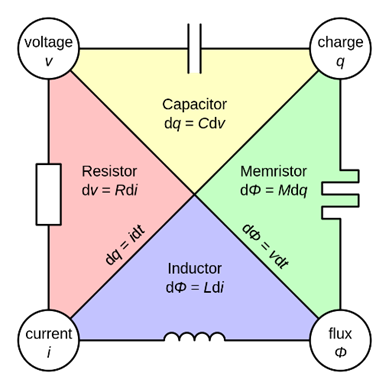
\includegraphics[width=0.5\textwidth]{Chapter1/Figs/1e.png}
    \caption[Conceptual symmetries of resistor, capacitor, inductor, and memristor]{Conceptual symmetries of resistor, capacitor, inductor, and memristor \cite{du2017metal}. These four fundamental variables in circuit theory are depicted with their relationships. Each variable can be related to another via either a passive component or a well-known equation.}
    \label{fig:1e}
\end{figure}

\noindent There are three fundamental circuit elements and four essential circuit variables in basic electrical circuit theory.  It is evident that one component is absent to achieve symmetry. This device ought to function in such a way that charge and magnetic flux are interconnected, as illustrated in Figure \ref{fig:1e}. The link between the mathematical memristive model and a two-terminal resistive switching device is pivotal in this instance. \\

\noindent The concept of memristance is distinct from that of resistance in that it is dependent on charge, rather than being a constant value.  The current is defined as the amount of charge flowing per unit time. Therefore, the expression for current can be written as:
\begin{align}
    q = \int_{-\infty}^{t_0} i(t)dt \label{eq:1.23}
\end{align}

\noindent where charge is the sum of current at a given time $t_0$.  \\

\noindent This indicates that the memristance, being dependent on charge, is determined by the historical currents that have previously passed through the device. In the event of interruption to the current flowing through the device, the memory state persists until the current flow is restored. The device is evidently equipped with a type of memory known as a "memristor".\\

\noindent In physical terms, memristors are often modeled as two-terminal devices whose resistance varies due to the drift of ions or vacancies in a dielectric medium. The state-dependent resistance can be written as:
\begin{align}
    V(t) = R(w(t)) \cdot I(t) \label{eq:1.24}
\end{align}

\noindent where $V(t)$ and $I(t)$ are the voltage and current at time $t$, $R(w(t))$ is the resistance depending on the internal state $w(t)$. This state $w(t)$ often represents physical quantities like oxygen vacancy concentration or filament length in resistive switching materials. $f(w, I) = \frac{dw}{dt}$ can be further defined as to how the internal state changes with input current. \\

\begin{figure}[htbp!] 
    \centering    
    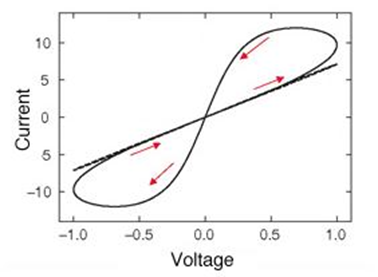
\includegraphics[width=0.5\textwidth]{Chapter1/Figs/1f.png}
    \caption[Typical I-V characteristic of a memristor]{The typical I-V characteristic  of a memristor displays a pinched hysteresis loop resulting from the nonlinear relationship between current and voltage in memristance \cite{wen2012dynamics}.}
    \label{fig:1f}
\end{figure}
    
\noindent From a visual standpoint, the pinched hysteresis loop, which is characteristic of the devices and dependent on frequency, distinguishes these memristor devices from other components \cite{chua2019resistance}, as shown in Figure \ref{fig:1f}. This loop represents a prevalent and inherent phenomenon in the natural world. It is evident that as the voltage input frequency increases, the loop undergoes a reduction in size. When the frequency approaches infinity, the memristor can be approximated as a resistor.\\

\noindent Among the range of new non-volatile memory devices, the primary focus of this study is on memristor devices, including MRAM, PRAM, FeRAM, and RRAM \cite{wang2017memristors}. Resistive switching, a reversible phenomenon of two-terminal elements, characterises the devices. Through electrical signalling, they change resistance in a non-volatile manner, with the process driving the resistive switching defined by the device's materials \cite{mehonic2018silicon}. \\

\noindent Resistive random-access memory (RRAM) is a device that uses resistance switching, where reversibility is attained through repeated application of appropriate stimuli, according to \cite{liu2010controllable}. Repeated application of suitable stimuli ensures reversibility. An RRAM cell comprises an insulating thin film (usually a metal oxide), sandwiched between two electrodes, within which resistance switching occurs. \\

\noindent The term "memristance" is favoured to express the general characteristics of these RRAM devices. The central hypothesis of this model is that memristance is a function of the total charge that has been passed through the device or that the integral of the applied voltage is consistent with certain experimental data. This can be used to toggle between different resistance levels. Although this ideal memristor model is often used in RRAM cells, it may not satisfy practical requirements. \\

% \begin{figure}[htbp!] 
%     \centering    
%     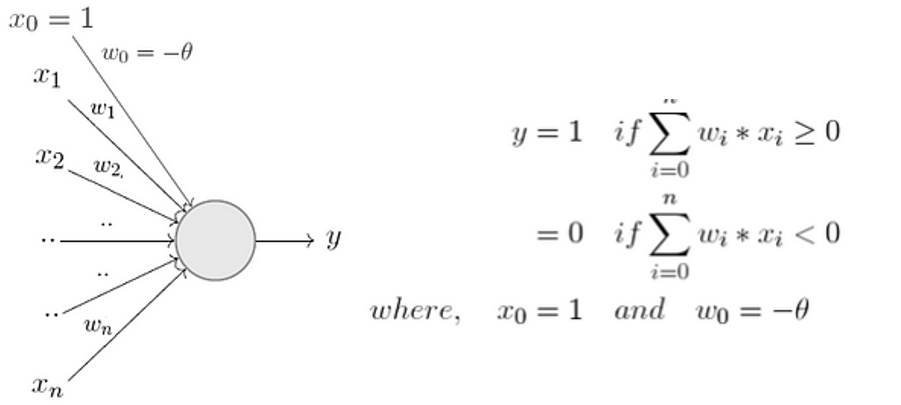
\includegraphics[width=0.8\textwidth]{Chapter1/Figs/1g.png}
%     \caption[The main RRAM types.]{The main RRAM types, from left to right: electrochemical metallization memory (ECM), vacancy change memory (VCM), and thermochemical memory (TCM). \cite{goux2016electrochemical}}
%     \label{fig:1g}
% \end{figure} 

\noindent Although all RRAM devices operate on a metal-insulator-metal (MIM) architecture, their categorisation and analysis remain challenging. RRAM devices are loosely classified into two types based on their functional mechanisms: oxide-RAM (OxRAM) and conductive bridge RAM (CBRAM) \cite{liu2015categorization}. \\

\noindent However, the internal physical behaviour of RRAM devices greatly varies, making it difficult to obtain a unified picture of them. RRAM cells may be classified according to their switching mechanisms which are electrochemical metallisation (ECM), valence change mechanism (VCM), or thermochemical mechanism (TCM) \cite{goux2016electrochemical}. \\

% The operation of the device is explained by one of the mechanisms depicted in Figure \ref{fig:1g}. \\

\noindent In normal operation, the state of the memristor can be objectively designated as having high resistance in the "OFF" state and low resistance in the "ON" state, with a substantial difference in resistance levels. The shift from the high resistance state (HRS) to the low resistance state (LRS) is referred to as "Set," while the reverse is called "Reset." An electroforming step is generally necessary to convert the device from pristine to switchable, whereby the former tends to exhibit higher resistance. \\

\noindent A hallmark of biorealistic learning is the ability to adjust synaptic strength continuously over time in response to neural activity. Analog (or gradual) switching in memristors is thus essential. Instead of binary ON/OFF transitions, these devices exhibit incremental conductance changes under controlled voltage pulse conditions. Consider a simplified state evolution model:
\begin{align}
    \frac{dw}{dt} = \mu \cdot I(t) \label{eq:1.25}
\end{align}
Where $\mu$ is a mobility parameter dependent on the device materials and structure. For voltage pulses of controlled amplitude and duration, this allows precise modulation of conductance:
\begin{align}
    \Delta G \varpropto \int I(t) dt = Q \label{eq:1.26}
\end{align}

\noindent Here, $Q$ is the total charge transferred, which accumulates over spike events. By shaping input pulses (in terms of rise time, width, or height), one can encode temporally-dependent plasticity rules such as STDP directly in hardware.\\

\noindent Despite their initial promise, memristive devices have been found to exhibit significant non-idealities \cite{govoreanu2013vacancy}. Device-to-device variability, encompassing factors such as conductance range, switching thresholds, and cycle-to-cycle behaviour, has the potential to vary across devices that appear to be nominally identical.\\

\noindent Non-linear phenomena, such as conductance updates, frequently exhibit saturation or asymmetric responses to positive and negative pulses. It is important to note that drift and retention loss, such as those occurring over time, may be attributable to the effects of relaxation. \\

\noindent To address these issues, neuromorphic systems often employ redundancy, error-tolerant learning algorithms, or closed-loop calibration techniques. Furthermore, some variability may be biologically realistic: synapses in the brain are not perfectly precise either, and stochasticity can enhance learning generalization and robustness.\\

\noindent For design and testing purposes, compact models of memristive devices are essential. These range from physics-based models to empirical abstractions. A popular framework is the linear ion drift model \cite{cai2011abel}, applicable to early $TiO_2$-based devices:
\begin{align}
    w(t) = w_0 + \frac{\mu_vR_{ON}}{D} \cdot \int_{0}^{t} I(\tau)   \,d\tau  \label{eq:1.27}
\end{align}

\noindent Where $\mu_v$ is the ion mobility, $R_{ON}$ is the low resistance state, $D$ is the device thickness. For practical simulations, window functions are often added to prevent unrealistic values of $w(t)$ outside the physical boundaries. A widely used modified form is:
\begin{align}
    \frac{dw}{dt} = \mu \cdot I(t) \cdot f(w) \label{eq:1.28}
\end{align}

\noindent Where $f(w)$ is a window function such as:
\begin{align}
    f(w) = 1 - (2w - 1)^{2p} \label{eq:1.29}
\end{align}
\noindent with $p$ controlling the non-linearity near the boundaries. These models allow researchers to prototype neuromorphic algorithms and circuits in software before hardware realization, enabling design-space exploration and validation under realistic conditions.


\subsection[In-memory Computing Paradigms]{In-memory Computing Paradigms}

\noindent Neuromorphic computing signifies a paradigm shift of the manner in which information is processed and stored; this is inspired directly by the architecture and function of biological neural systems. Conventional computing systems compartmentalise memory and processing units, a configuration that engenders energy and velocity inefficiencies due to incessant data movement. Neuromorphic systems are designed to co-locate memory and computation by leveraging distributed, parallel architectures that emulate the brain's functionality.\\

\noindent The origin of neuromorphic engineering can be traced to the pioneering work of Carver Mead in the 1980s \cite{mead1989analog}, who proposed using analog electronics to mimic the function of neurons and synapses. Since then, the field has grown to encompass both analog and digital implementations of brain-inspired circuits.\\

\noindent The fundamental principle of neuromorphic computing is the translation of key neurobiological principles into hardware. Event-driven processing is a key feature of neuromorphic circuits, which, like biological neurons, only activate when necessary, thereby significantly reducing power consumption. \\

\noindent As an illustrative example, synapses (which are implemented by resistive memory elements) function as both computational units and memory stores. Neuromorphic systems have been demonstrated to exhibit plasticity and the capacity for real-time, local learning through the utilisation of biologically plausible rules, such as the STDP (synaptic tagging with depolarisation-dependent plasticity) rule. \\

\noindent Neuromorphic architectures can be broadly classified into two categories \cite{ceolini2020hand}. Digital neuromorphic systems are comprised of digital circuits which simulate the behaviour of neurons, i.e. their spiking. Notable examples of this include IBM's TrueNorth and Intel's Loihi. These chips implement large networks of spiking neurons with programmable connectivity and plasticity. Analog/Mixed-Signal Systems have been shown to exhibit a greater degree of similarity to the continuous dynamics of biological neurons and synapses. Memristive arrays frequently fall into this category, offering a physical substrate for analogue computation.\\

\begin{figure}[htbp!] 
    \centering    
    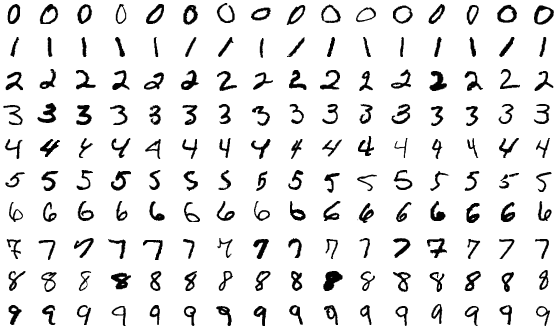
\includegraphics[width=0.5\textwidth]{Chapter1/Figs/1h.png}
    \caption[The memristor-based crossbar architecture.]{The memristor-based crossbar architecture with a single memristor array and a constant-term circuit \cite{truong2014new}. The resistive components are located at the connections of the word and bit lines. When voltages $\mathbf{V}$ are applied to the word line, the resistive element at the junction of the $i^{th}$ word line and the $j^{th}$ bit line generates $V_i \times G_{i,j}$ units of current, assuming zero wire resistance, as per Ohm's law. The currents created by each individual element are then aggregated along the bit lines using Kirchhoff's current law.}
    \label{fig:1h}
\end{figure}
    

\noindent A key architectural unit is the crossbar array, in which vertical and horizontal metal lines intersect at memristive devices. This structure supports efficient matrix-vector multiplication—the fundamental operation in neural networks. Let $V$ be a voltage vector applied to input rows, and $G$ be the conductance matrix of memristive elements. The output current vector $I$ on the columns is given by:
\begin{align}
    \mathbf{I} = \mathbf{G} \cdot \mathbf{V} \label{eq:1.30}
\end{align}

\noindent This analog computation occurs in a single step without requiring data movement between separate processing and memory units, thus offering significant energy efficiency. Linear algebra and vector-matrix products rely heavily on multiplication and addition. These procedures can be carried out by using fundamental circuit laws. \\

\noindent Consider a resistive element with conductance $G$ (the reciprocal of resistance). If a voltage $V$ is supplied to it, the current $I$ flowing through it will be equal to $V \times G$. This indicates that conductance $G$ functions as a multiplicative factor, as per Ohm's law. For a circuit with several branches, each carrying a current $I_i$. At the intersection of these branches, the total current flowing through it will be $I = \sum_{i}^{} I_i$. This indicates that currents are combined together, as per Kirchhoff's current law. \\

\noindent Once multiplication and addition are possible, higher-level operations may be performed using specialist circuits. For vector-matrix products, a resistive crossbar array can be used, which is a two-dimensional grid of conductive wires with resistive components at each intersection. A crossbar array's output currents are essentially the product of a voltage vector and a conductance matrix. Consider a vector-matrix product, $\mathbf{y} = \mathbf{x}^\intercal \mathbf{W}$. Where $\mathbf{x}$ can be translated to voltages $\mathbf{V} = k_V\mathbf{x}$, $\mathbf{W}$ to conductances $\mathbf{G} = k_G \mathbf{W}$, and generate outputs $\mathbf{y}$ from currents $\mathbf{I} = \mathbf{y} k_V k_G $, where $k_V$ and $k_G$ are positive constants. \\


\noindent Crossbars can compute products of voltage vectors and conductance matrices due to their structural design. This is because the structure controls which voltage-conductance pairs are multiplied and which consequent currents are combined together. These circuits have two sets of wires: word lines and bit lines. Voltages $\mathbf{V}$ are applied to the word lines, and currents $\mathbf{I}$ are measured along the bit lines. A resistive element located at the junction of the $i^{th}$ word line and the $j^{th}$ bit line has a conductance of $G_{i,j}$.\\
    
\noindent When $V_i$ is applied to the $i^{th}$ word line, the device generates a current of $V_i \times G_{i,j}$ (assuming no wire resistance). The currents generated in the jth bit line are added together to provide a current of $I_j$. This current is calculated by taking the dot product of voltage $\mathbf{V}$ and the $j^{th}$ column of the conductance matrix $\mathbf{G}$. Given that the $j^{th}$ element of a vector-matrix product is just the dot product of the vector and the $j^{th}$ column of the matrix, the vector containing all output currents may be concisely expressed as $\mathbf{I}^\intercal = \mathbf{V}^\intercal \mathbf{G}$. \\
    
\noindent The individual application determines which resistive devices are used in the crossbar array. Weights $\mathbf{W}$ are repeatedly updated during neural network training, necessitating the ability to alter the conductances in the crossbar array numerous times. In contrast, during inference, the weights are fixed, allowing the conductances to be set after initial programming. Regardless of the conditions, the conductances will be unique to the network, requiring the ability to change them at least once. \\
    
\noindent Memristive devices, or memrisitors, are differentiated by their ability to change their conductance in response to electrical inputs. As a result, they make an excellent choice for crossbar-based linear algebra accelerators. The choice of memristor depends on whether the crossbar array is used for training or inference. The former is far more difficult and would demand memristors that can be repeatedly programmed in a linear fashion. Given these complications, much research on memristive crossbars has been on inference. \\
    
\noindent Even in the absence of nonidealities, any memristor will have a restricted range of conductance values that it can be configured to. This is a hurdle when attempting to represent real numbers with solely positive conductances $G$. To demonstrate, if the range of attainable conductances is $G \in [G_{off}, G_{on}]$, the crossbar array can only represent matrix values up to $w \in \left [ \frac{G_{off}}{k_G}, \frac{G_{on}}{k_G} \right ]$. Since $G_{off}$ is a positive number, hence only positive $w$ may be expressed. \\
    
\noindent One potential option is to employ differential pairs, in which the matrix element $w$ is represented as the difference between two conductances, $G+$ and $G-$ \cite{joksas2022nonideality}. The two conductances can be chosen symmetrically around the 'average' value $G \pm = G_{avg} \pm \frac{k_G w}{2}$, where $G_{avg} = \frac{G_{off} + G_{on}}{2}$. The two sets of conductances can be represented by independent conductance matrices $\mathbf{G}+$ and $\mathbf{G}-$, which are assigned to different bit lines of the crossbar array \cite{kim20214k}. \\
    
\noindent The bit lines will then generate independent sets of currents, which may be represented as vectors $\mathbf{I}+$ and $\mathbf{I}-$. Vector-matrix products are linear, thus the result may be calculated by subtracting $\mathbf{I}-$ from $\mathbf{I}+$. In reality, the 'positive' and 'negative' bit lines are frequently arranged near to one another, which helps to mitigate the detrimental effects of line resistance, a significant non-ideality \cite{joksas2020committee}. \\

% \noindent Unlike traditional artificial neural networks (ANNs), which use continuous-valued activations, SNNs operate using discrete spikes, more closely resembling biological neurons. In SNNs, information is encoded not in the magnitude of activation but in the timing and frequency of spikes—a paradigm known as temporal coding. \\

% \noindent The dynamic state of a spiking neuron evolves according to differential equations such as those in the LIF model described in previous section. Networks of such neurons can perform complex computations, including pattern recognition, signal processing, and control tasks.\\

% SNNs are particularly well-suited for implementation on neuromorphic hardware due to their:

% Sparsity: Most neurons are inactive at any given time, reducing energy consumption.

% Locality: Updates and communication occur between neighboring units, minimizing global data traffic.

% Temporal Processing: Inherent ability to handle time-series data and asynchronous signals.

\noindent The learning process in neuromorphic systems can be categorised into three distinct approaches: supervised learning, unsupervised learning, and reinforcement-based learning \cite{stone2019artificial}. Nevertheless, with respect to biorealistic implementation, unsupervised, local learning is most aligned with the biological model. \\

\noindent Biorealistic learning draws upon the empirical laws of synaptic plasticity observed in biological systems. Central among these are Hebbian Learning \cite{kempter1999hebbian} which stated "Neurons that fire together wire together." This principle is often expressed in simplified form as:\\
\begin{align}
    \Delta w_{ij} = \eta \cdot x_i \cdot y_i \label{eq:1.31}
\end{align}

\noindent Where $\Delta w_{ij}$ is the change in synaptic weight between pre-synaptic neuron $i$ and post-synaptic neuron $j$, $x_i$ and $y_i$ are the activity levels of the respective neurons, $\eta$ is the learning rate. \\

\noindent Hebbian learning is predicated on the premise that the strength of a synapse is enhanced by co-activity between pre- and post-synaptic neurons \cite{frenkel2019morphic}. Alternatively, STDP is atemporally-sensitive variant of Hebbian learning, a concept that has already been covered in the preceding section. Homeostatic plasticity is a global mechanism that ensures that overall neural activity remains within functional bounds. This is analogous to metabolic regulation in biology.\\

\noindent These mechanisms are often implemented using local circuit rules. For instance, in memristive implementations of STDP, pulse timing determines the net change in conductance of a memristor. The result is a physical device whose behavior embodies the learning rule itself. In digital systems, learning involves weight updates of the form:
\begin{align}
    w_{ij} \leftarrow w_{ij} + \eta \cdot \delta_j \cdot x_i \label{eq:1.32} 
\end{align}

\noindent Where $w_{ij}$ is the synaptic weight from neuron $i$ to neuron $j$, $\eta$ is the learning rate, $\delta_j$ is the error signal at the output neuron $j$, and $x_i$ is the activation of input neuron $i$. In contrast, memristive learning avoids explicit error backpropagation and instead uses local learning rules where the change in conductance $\Delta G$ depends on spike-timing and voltage:
\begin{align}
    \Delta G \varpropto f(\Delta t_{ij}) \cdot g(V_{pre}, V_{post}) \label{eq:1.33}
\end{align}

\noindent Here, $f(\Delta t_{ij})$ reflects the STDP window and $g(V_{pre}, V_{post})$ models the effect of voltage pulses on device conductance. Memristors thus act as "plastic synapses" whose weights evolve in real time, guided by the temporal correlation of pre- and post-synaptic activity.

\subsection[Encoding Plasticity in Memristors]{Encoding Plasticity in Memristors}

As neuromorphic systems aspire to emulate biological intelligence, the implementation of biorealistic learning—learning mechanisms that faithfully reproduce the behavior of biological synapses and neurons—has become central to the development of memristor-based architectures. This section explores how learning rules inspired by neuroscience, such as spike-timing-dependent plasticity (STDP), Hebbian learning, and homeostatic regulation, can be embedded into memristive networks.\\

\noindent To implement STDP and other plasticity rules in hardware, researchers have developed pulse-pairing schemes that encode spike timing as overlapping voltage pulses applied to memristive synapses. These rules can be implemented physically using the conductance modulation behavior of memristors, which act as artificial synapses \cite{campbell2016pulse}. \\

\noindent For instance, a presynaptic spike instigates a positive voltage pulse, whereas a postsynaptic spike precipitates a negative voltage pulse. The net voltage across the memristor depends on the temporal alignment of these spikes. If the pulses overlap constructively (e.g., pre before post), the net voltage exceeds a potentiation threshold, increasing conductance. If the order is reversed (post before pre), the net voltage may trigger depression. \\

\noindent Let the pulse shape be $V_{pre}(t)$ and $V_{post}(t)$, The effective voltage across the memristor is:
\begin{align}
    V_{mem}(t) = V_{pre}(t) - V_{post}(t) \label{eq:1.34}
\end{align}

\noindent Depending on $ V_{mem}(t)$, the conductance $G(t)$ changes according to a windowed integration rule, often expressed as:
\begin{align}
    \Delta G = \int_{-\infty}^{-\infty} \gamma (V_{mem}(t)) \,dt \label{eq:1.35}
\end{align}
\noindent Where $\gamma(\cdot)$ is a non-linear function mapping voltage to conductance change. \\

\noindent At the network scale, memristive synapses form dense connectivity graphs akin to biological networks. When configured with spiking neurons, the resulting system exhibits emergent learning behavior. A typical learning architecture may include a spiking neural network (SNN) layer of leaky integrate-and-fire (LIF) neurons, memristive crossbar arrays that implement synaptic weights, spike-based learning circuits that detect relative spike timing and apply appropriate pulses.\\

\noindent Mathematically, for a neuron receiving inputs $x_i(t)$ through synapses $G_i(t)$, the membrane potential $V_m$ evolves as:
\begin{align}
    C_m \frac{dV_m}{dt} = -\frac{V_m}{R_m} + \sum_{i} G_i(t) \cdot x_i(t) \label{eq:1.36}
\end{align}

\noindent Where $C_m$ and $R_m$ are are the membrane capacitance and leakage resistance respectively. When $V_m$ exceeds a threshold $V_th$, the neuron spikes and resets. Synaptic updates follow:
\begin{align}
    \Delta G_i(t) = f(\Delta t_i) \cdot Pulse_{pairing}(x_i(t), y(t)) \label{eq:1.37}
\end{align}

\noindent With $f(\Delta t_i)$ as an STDP kernel and $Pulse_{pairing}$ as the hardware-driven pulse overlap function.

\noindent An illustrative application of biorealistic learning is unsupervised pattern recognition. For instance, when exposed to MNIST digit images encoded as spiking input, memristive networks have been shown to learn digit prototypes using STDP.\\

\noindent In such systems, Each input pixel is connected to neurons through memristive synapses. The input is converted to spike trains based on intensity. Competitive mechanisms such as winner-take-all inhibit multiple neurons from firing simultaneously. STDP strengthens synapses associated with active neurons and temporally correlated inputs. Over time, distinct neurons specialize in responding to specific digit patterns, emulating feature selectivity observed in biological cortical areas.\\

\noindent Unbounded synaptic growth has the potential to destabilise learning. It is evident that biological systems utilise homeostatic mechanisms in order to maintain equilibrium between synapses and network stability. It is therefore imperative to acknowledge that analogous mechanisms are indispensable in memristive networks. \\

\noindent Synaptic normalization is a common strategy that involves the enforcement of a constraint so that the sum of synaptic weights for a neuron remains constant:
\begin{align}
    \sum_{i} G_i = G_{max} \label{eq:1.38}
\end{align}

\noindent Alternatively, weight decay is used to gradually reducing all synaptic weights over time, modeling biological forgetting:
\begin{align}
    G_i(t + \Delta t) = (1 - \alpha) \cdot G_i(t) + \Delta G_i \label{eq:1.39}
\end{align}

\noindent Where $\alpha$ is a small decay factor. These mechanisms ensure that learning remains stable over long durations, enabling continual learning without catastrophic forgetting.

\section[Architectures and System-Level Integration]{Architectures and System-Level Integration}

\noindent Memristive networks offer distinct advantages. The elimination of the von Neumann bottleneck by in-memory learning is a significant development in this field. The subthreshold operation enables ultra-low-power computation, while the physical time integration closely matches biological computation timescales. \\

\noindent Nevertheless, challenges persist. It is important to note that variability and inconsistent device behaviour have the capacity to disrupt precise learning rules. Furthermore, write endurance on devices may degrade under repeated programming, and non-linear dynamics with real devices often do not match idealised learning models.\\

\noindent Notwithstanding these challenges, the co-design of algorithms and devices, whereby learning rules are adapted to the characteristics of the device, facilitates the practical implementation of biorealistic learning paradigms.\\

\noindent While individual memristive synapses provide the foundational building blocks for biorealistic learning, realizing practical neuromorphic systems requires architectural integration at scale. This section explores how memristive networks are organized into hierarchical architectures, interfaced with complementary computing modules, and optimized for system-level performance. The goal is to demonstrate how the principles of biology-inspired learning translate into cohesive hardware systems that support advanced computation.

\subsection[Hierarchical Modular Architectures]{Hierarchical Modular Architectures}

\subsection[Hardware-Software Co-Design]{Hardware-Software Co-Design}

\subsection[Experimental Validations Structure]{Experimental Validations Structure}

\section[Summary]{Summary}